\documentclass[crop]{standalone}

\usepackage[dvipsnames]{xcolor}
\usepackage{tikz}

\usetikzlibrary{backgrounds}

\begin{document}
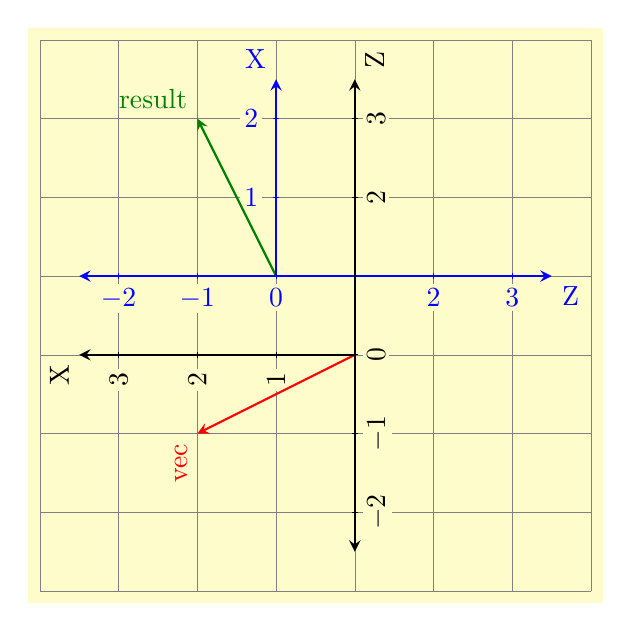
\begin{tikzpicture}[background rectangle/.style={fill=yellow!20}, show background rectangle, rotate=90,transform shape]


	\draw[step=1cm,gray,very thin] (-3,-3) grid (4,4);

	\foreach \z in {-2,-1,0,2,3}
		\draw (\z cm,1pt) -- (\z cm,-1pt) node[anchor=north, inner sep=1.5pt, outer ysep=2pt, fill=yellow!20] {$\z$};
	\foreach \x in {1,2,3}
		\draw (1pt,\x cm) -- (-1pt,\x cm) node[anchor=east, inner sep=1.5pt, outer xsep=4pt, fill=yellow!20] {$\x$};

	% Usin' coordinate transforms to explain coordinate transforms
	\begin{scope}[shift={(1,1)},rotate=-90,blue,transform shape]
		\foreach \z in {-2,-1,0,2,3}
			\draw (\z cm,1pt) -- (\z cm,-1pt) node[anchor=north, inner sep=1.5pt, outer ysep=2pt, fill=yellow!20] {$\z$};
		\foreach \x in {1,2}
			\draw (1pt,\x cm) -- (-1pt,\x cm) node[anchor=east, inner sep=1.5pt, outer xsep=4pt, fill=yellow!20] {$\x$};
	\end{scope}

	\draw[thick,-stealth,red] (0,0) -- (-1,2) node[anchor=south east] {vec};
	\begin{scope}[shift={(1,1)},rotate=-90,transform shape]
		\draw[thick,-stealth,Green] (0,0) -- (-1,2) node[anchor=south east] {result};
	\end{scope}

	\begin{scope}[shift={(1,1)},rotate=270,blue,transform shape]
		\draw[thick,stealth-stealth] (-2.5,0) -- (3.5,0) node[anchor=north west] {Z};
		\draw[thick,-stealth] (0,0) -- (0,2.5) node[anchor=south east] {X};
	\end{scope}

	\draw[thick,stealth-stealth] (-2.5,0) -- (3.5,0) node[anchor=north west] {Z};
	\draw[thick,-stealth] (0,0) -- (0,3.5) node[anchor=south east] {X};


\end{tikzpicture}
\end{document}
